\section{Related Work}

\label{sec:related}
\renewcommand{\thesubsection}{\Alph{subsection}}   
\renewcommand{\thesection}{\arabic{section}}       
Time series forecasting is the process of generating a future segment of a time series by applying specific time series forecasting algorithms to historical time series data. For example, as shown in Figure 1, a historical wind speed series of 100 time units is used to generate a future wind speed series of 50 time units.Time series forecasting has undergone three evolutionary phases: statistical modeling, deep learning revolution, and the emerging diffusion paradigm. We critically analyze these paradigms with a focus on their capabilities and limitations.

\begin{figure*}[!ht]
\centering
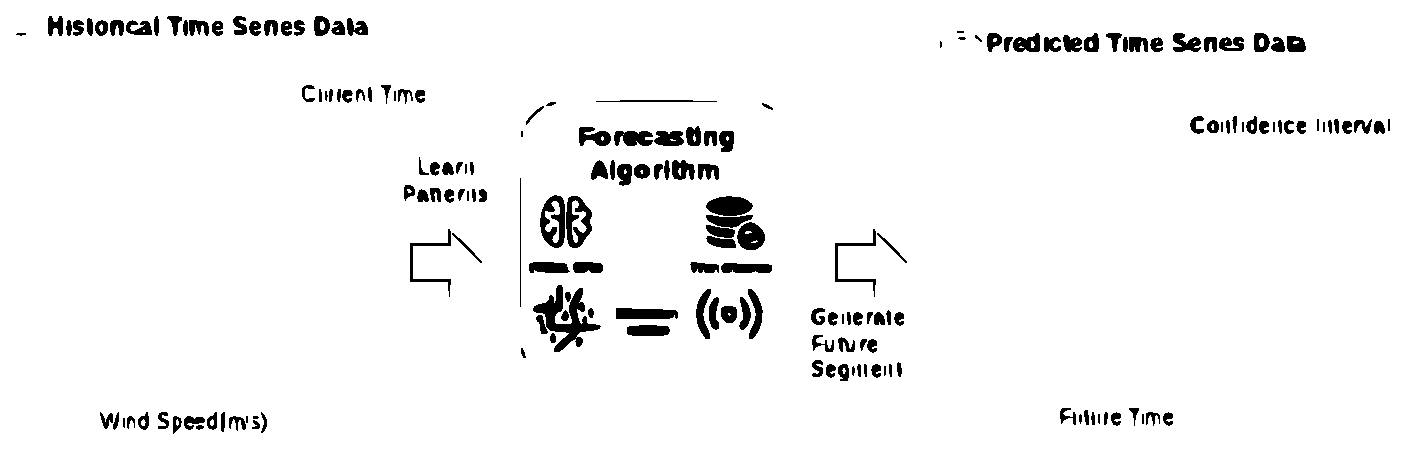
\includegraphics[width=0.9\linewidth]{figures/Slide1}
\caption{Time series forecast}
\label{fig:qualitative}
\end{figure*}


% Please add the following required packages to your document preamble:
% \usepackage{multirow}

% \begin{table*}[!ht]
% 	\centering
% 	{\small\scriptsize
% 		\caption{\small Comparative Analysis of Time Series Forecasting Approaches} \label{tab:method_comparison}
% 		\resizebox{\textwidth}{!}{ % 宽度设为文本宽度,高度按比例缩放
% 			\begin{tabular}{|c|c|c|c|c|c|c|c|}
% 				\hline
% 				Paradigm                                 & Method             & Model/Technique                                  & Variable-Length Support & Multi-Scale Modeling          & Key Innovations                                                        & Limitations \& Challenges                                   &                                        \\ \hline
% 				\multirow{4}{*}{Traditional Statistical} & ARIMA/SARIMA       & Auto-regressive + Moving Average + Differencing  & No                      & No                            & Handles linear trends and seasonality                                  & Only works for stationary linear data                       & fails on complex nonlinear patterns    \\ \cline{2-8} 
% 				& VAR                & Vector Auto-regression                           & No                      & No                            & Multivariate joint modeling                                            & Computational complexity grows exponentially with variables &                                        \\ \cline{2-8} 
% 				& Holt-Winters       & Triple Exponential Smoothing                     & No                      & Partial (Seasonal only)       & Intuitive trend-seasonality decomposition                              & Requires predefined seasonal period parameters              &                                        \\ \cline{2-8} 
% 				& Gaussian Processes & Kernel-based temporal modeling                   & Yes                     & No                            & Probabilistic forecasting with uncertainty quantification              & Sensitive to kernel choice                                  & computationally expensive for big data \\ \hline
% 				\multirow{6}{*}{Deep Learning}           & LSTM/GRU           & Gated Recurrent Networks                         & Yes                     & No                            & Solves long-term dependency problems                                   & Difficult to parallelize                                    & gradient vanishing in long sequences   \\ \cline{2-8} 
% 				& DeepAR             & Auto-regressive LSTM + Probabilistic output      & No                      & No                            & Probabilistic time series forecasting                                  & Slow autoregressive generation                              & error accumulation                     \\ \cline{2-8} 
% 				& WaveNet/TCN        & Dilated Causal Convolutions                      & Yes                     & Partial (Depends on dilation) & Parallel training and long-range capture                               & Receptive field limited by dilation rates                   & high memory usage                      \\ \cline{2-8} 
% 				& Transformer        & Self-attention mechanism                         & Yes                     & No                            & Global dependency modeling                                             & O(n²) computational complexity                              & struggles with long sequences          \\ \cline{2-8} 
% 				& Informer           & Sparse Attention                                 & Yes                     & No                            & Reduces attention computation complexity                               & Sparse patterns may lose local details                      &                                        \\ \cline{2-8} 
% 				& Autoformer         & Auto-correlation mechanism                       & Yes                     & Partial (Seasonal decomp)     & Frequency-domain time series modeling                                  & Requires predefined seasonal periods                        &                                        \\ \hline
% 				\multirow{6}{*}{Diffusion Models}        & TimeGrad           & Diffusion process + RNN conditioning             & No                      & No                            & First TS diffusion framework                                           & Slow autoregressive generation                              & no variable-length support             \\ \cline{2-8} 
% 				& CSDI               & Conditional score-based diffusion                & No                      & No                            & Unified imputation and forecasting                                     & Dual Transformer architecture computationally expensive     &                                        \\ \cline{2-8} 
% 				& SSSD               & Structured State Space + Diffusion               & Yes                     & No                            & Continuous-time modeling and efficient long-range capture              & State space dimensions require tuning                       &                                        \\ \cline{2-8} 
% 				& TSDiff             & Time-series-as-image representation              & Yes                     & No                            & Variable-length input handling                                         & 2D representation may disrupt temporal locality             &                                        \\ \cline{2-8} 
% 				& DiffSTG            & Graph Neural Network + Diffusion                 & No                      & No                            & Spatio-temporal graph structure modeling                               & Graph construction relies on prior knowledge                &                                        \\ \cline{2-8} 
% 				& mr-Diff      & Multi-resolution trend decomposition + Diffusion & Yes                     & Yes                           & Explicit multi-scale modeling \& progressive coarse-to-fine generation & High training complexity from multi-stage approach          &                                        \\ \hline
% 			\end{tabular}
% 		 }
% 	}\vspace{-2ex}
% \end{table*}







\subsection{Statistical and Classical Machine Learning Methods}
Early approaches to time series forecasting primarily relied on explicit statistical assumptions about temporal dependencies and noise distributions.

Linear models such as the Autoregressive Integrated Moving Average (ARIMA) model [1] have long dominated classical forecasting, offering interpretable formulations under stationarity and linearity assumptions. Its seasonal variant, SARIMA, further extends the framework to capture periodic fluctuations. The Vector Autoregression (VAR) model [2] generalizes these ideas to the multivariate setting, enabling linear inter-series dependency modeling across multiple correlated variables.

Beyond parametric formulations, nonparametric smoothing methods such as the Holt–Winters exponential smoothing [3] empirically model trend–seasonality interactions without requiring strong distributional assumptions. The Error–Trend–Seasonality (ETS) framework [4] unifies these techniques by decomposing time series into interpretable components under a state-space representation, supporting both additive and multiplicative structures.

From a probabilistic perspective, Gaussian Process (GP) models [5] introduced a Bayesian approach to time series prediction, providing principled uncertainty quantification through kernel-based covariance functions. These models capture local smoothness and uncertainty propagation effectively in low-dimensional settings.

% \begin{itemize}
% 	\item \textbf{Linear Models}:
% 	\begin{itemize}
% 		\item ARIMA \cite{2013ARIMA} dominated linear time series analysis, with SARIMA extending to seasonal data
% 		\item VAR \cite{Zivot2003} introduced multivariate linear dependence
% 	\end{itemize}
	
% 	\item \textbf{Nonparametric Smoothing}:
% 	\begin{itemize}
% 		\item Holt-Winters \cite{KOEHLER2001269} empirically captured trend-seasonality interactions
% 		\item ETS framework \cite{RePEc:bla:istatr:v:77:y:2009:i:2:p:315-316} provided a unified error-trend-seasonality formulation
% 	\end{itemize}
	
% 	\item \textbf{Probabilistic Approaches}:
% 	\begin{itemize}
% 		\item Gaussian Processes \cite{2005Gaussian} enabled Bayesian uncertainty quantification
% 	\end{itemize}
% \end{itemize}

However, despite their interpretability and strong theoretical grounding, these statistical methods struggle to model nonlinear, nonstationary, and high-dimensional temporal dynamics common in modern real-world applications.Their reliance on fixed functional forms and limited scalability restricts their ability to capture complex dependencies and long-range interactions, motivating the transition toward deep learning and generative paradigms in subsequent research.

\subsection{Deep Learning Revolution}
The emergence of neural networks has fundamentally transformed time series forecasting by enabling hierarchical feature learning and nonlinear temporal dependency modeling. Unlike statistical approaches with fixed assumptions, neural networks learn dynamic representations directly from data, capturing complex interactions across multiple time scales.

%\subsubsection{Sequential Modeling}
% \begin{itemize}
% 	\item LSTM \cite{6795963} overcame gradient vanishing via gated mechanisms
% 	\item GRU \cite{2014Learning} simplified gating while preserving performance
% 	\item DeepAR \cite{2020DeepAR} integrated autoregressive LSTMs with probabilistic outputs
% \end{itemize}

% \subsubsection{Parallelizable Architectures}
% \begin{itemize}
% 	\item WaveNet \cite{2016WaveNet} used dilated convolutions for long-range dependencies
% 	\item TCNs \cite{2018Trellis} established residual connections for efficient training
% \end{itemize}

% \subsubsection{Attention-Based Paradigms}
% \begin{itemize}
% 	\item Transformer \cite{2017Attention} enabled global dependency modeling via self-attention
% 	\item Informer \cite{2020Informer} addressed quadratic complexity through sparse attention
% 	\item Autoformer \cite{2021Autoformer} replaced attention with frequency-domain autocorrelation
% \end{itemize}

Early sequential architectures such as the Long Short-Term Memory (LSTM) network [6] addressed the vanishing gradient problem through gated mechanisms that preserve long-term information, while the Gated Recurrent Unit (GRU) [7] simplified this structure to enhance computational efficiency with comparable accuracy. Building on these foundations, DeepAR [8] combined autoregressive likelihood estimation with LSTM encoders, establishing a deep probabilistic framework for multivariate time series forecasting.

To overcome the sequential bottleneck of recurrent networks, convolution-based models such as WaveNet [9] and Temporal Convolutional Networks (TCNs) [10] employed dilated causal convolutions and residual connections to capture long-range dependencies in a fully parallelizable manner. These architectures marked a shift from sequential recurrence to efficient hierarchical temporal modeling.

More recently, attention-based architectures have advanced forecasting by modeling global temporal dependencies. The Transformer [11] introduced self-attention to directly capture long-range interactions, achieving strong performance across diverse sequence tasks. Its variants, Informer [12] and Autoformer [13], further improved efficiency and interpretability through sparse attention and frequency-domain autocorrelation, respectively, making attention mechanisms a dominant paradigm in long-horizon time series forecasting.

\subsection{Diffusion Models in Time Series}
Building on deep learning successes, diffusion models have emerged as powerful generative tools:recent research has shifted toward generative frameworks that model the full predictive distribution of time series rather than point estimates. TimeGrad [14] first introduced autoregressive denoising diffusion for multivariate probabilistic forecasting, demonstrating the ability of diffusion models to capture uncertainty through iterative noise refinement. CSDI [15] extended this idea with conditional score-based diffusion, enabling flexible handling of missing observations and context-aware forecasting. Subsequent methods incorporated learned guidance, hybrid backbones, and structured state-space formulations [16–17] to improve sampling efficiency and capture long-range temporal dependencies.
\vspace{-15pt}
\begin{table}[htbp]
\caption{Comparison of different time-series methods}
\begin{tabular}{@{}lcc@{}}
\toprule
\textbf{Method} & \textbf{Var.-Len.} & \textbf{Multi-Scale} \\
\midrule
\multicolumn{3}{@{}l}{\textit{Traditional Statistical}} \\
\quad ARIMA/SARIMA & $\times$ & $\times$ \\
\quad VAR            & $\times$ & $\times$ \\
\quad Holt-Winters   & $\times$ & $\times$ (seasonal) \\
\quad Gaussian Proc. & $\checkmark$ & $\times$ \\
\quad LSTM/GRU       & \checkmark & $\times$ \\
\quad DeepAR         & $\times$ & $\times$ \\
\midrule
\multicolumn{3}{@{}l}{\textit{Deep Learning}} \\
\quad WaveNet/TCN    & \checkmark & \checkmark$^\dag$ \\
\quad Transformer    & \checkmark & $\times$ \\
\quad Informer       & \checkmark & $\times$ \\
\quad Autoformer     & \checkmark & \checkmark$^\dag$ \\
\quad TimeGrad       & $\times$ & $\times$ \\
\midrule
\multicolumn{3}{@{}l}{\textit{Diffusion Models}} \\
\quad CSDI           & $\times$ & $\times$ \\
\quad SSSD            & \checkmark & $\times$ \\
\quad TSDiff          & \checkmark & $\times$ \\
\quad DiffSTG         & $\times$ & $\times$ \\
\quad \textbf{ours} & $\boldsymbol{\checkmark}$ & $\boldsymbol{\checkmark}$ \\ 
\bottomrule
\smallskip
{\small $^\dag$ Depends on dilation / seasonal decomposition.}
\end{tabular}
\end{table}


% \subsubsection{Foundational Works}
% \begin{itemize}
% 	\item TimeGrad \cite{2021Autoregressive} combined diffusion with RNN-based conditioning
% 	\item CSDI \cite{2021CSDI} adapted score-based diffusion for missing value imputation
% \end{itemize}

% \subsubsection{Architectural Innovations}
% Recent advances address key limitations:
% \begin{itemize}
% 	\item SSSD \cite{alcaraz2022diffusion} integrated state space models for efficient long-range modeling
% 	\item TSDiff \cite{naiman_utilizing_nodate} encoded variable-length series as 2D representations
% 	\item DiffSTG \cite{10.1145/3589132.3625614} incorporated graph structures for spatio-temporal data
% 	\item mr-Diff \cite{shen_multi-resolution_2024} pioneered multi-scale decomposition via seasonal-trend analysis
% \end{itemize}


\vspace{-15pt}


\textbf{Critical Gap:} Existing diffusion approaches exhibit three key limitations,which reflected in the Table 1: 
(1) rigidity in handling variable-length inputs, 
(2) absence of explicit multi-scale modeling, and 
(3) computational inefficiency in inference. 

Our framework addresses these challenges through three key designs: an adaptive delay embedding for variable-length inputs, a hierarchical multi-resolution decomposition to model temporal patterns across scales, and a conditionally guided diffusion process that leverages coarse trends to enhance efficiency and stability.










